% CVPR 2026 Paper Template; see https://github.com/cvpr-org/author-kit

\documentclass[10pt,twocolumn,letterpaper]{article}

%%%%%%%%% PAPER TYPE  - PLEASE UPDATE FOR FINAL VERSION
% \usepackage{cvpr}              % To produce the CAMERA-READY version
% \usepackage[review]{cvpr}      % To produce the REVIEW version
\usepackage[pagenumbers]{cvpr} % To force page numbers, e.g. for an arXiv version

% Import additional packages in the preamble file, before hyperref
%% This file contains a number of tweaks that are typically applied to the main document.
%% They are not enabled by default, but can be enabled by uncommenting the relevant lines.

%%
%% Inline annotations; for predefined colors, refer to "dvipsnames" in the xcolor package:
%% https://tinyurl.com/overleaf-colors
%%
\newcommand{\red}[1]{{\color{red}#1}}
\newcommand{\todo}[1]{{\color{red}#1}}
\newcommand{\TODO}[1]{\textbf{\color{red}[TODO: #1]}}
%%
%% disable for camera ready / submission by uncommenting these lines  
%%
% \renewcommand{\TODO}[1]{}
% \renewcommand{\todo}[1]{#1}

%%
%% work harder in optimizing text layout. Typically shrinks text by 1/6 of page, enable
%% it at the very end of the writing process, when you are just above the page limit
%%
% \usepackage{microtype}

%%
%% fine-tune paragraph spacing
%%
% \renewcommand{\paragraph}[1]{\vspace{.5em}\noindent\textbf{#1.}}

%%
%% globally adjusts space between figure and caption
%%
% \setlength{\abovecaptionskip}{.5em}


%%
%% Allows "the use of \paper to refer to the project name"
%% with automatic management of space at the end of the word
%%
% \usepackage{xspace}
% \newcommand{\paper}{ProjectName\xspace}

%%
%% Commonly used math definitions
%%
% \DeclareMathOperator*{\argmin}{arg\,min}
% \DeclareMathOperator*{\argmax}{arg\,max}

%%
%% Tigthen underline
%%
% \usepackage{soul}
% \setuldepth{foobar}

% It is strongly recommended to use hyperref, especially for the review version.
% hyperref with option pagebackref eases the reviewers' job.
% Please disable hyperref *only* if you encounter grave issues, 
% e.g. with the file validation for the camera-ready version.
%
% If you comment hyperref and then uncomment it, you should delete *.aux before re-running LaTeX.
% (Or just hit 'q' on the first LaTeX run, let it finish, and you should be clear).
\definecolor{cvprblue}{rgb}{0.21,0.49,0.74}
\usepackage[pagebackref,breaklinks,colorlinks,allcolors=cvprblue]{hyperref}

%%%%%%%%% PAPER ID  - PLEASE UPDATE
\def\paperID{*****} % *** Enter the Paper ID here
\def\confName{CVPR}
\def\confYear{2026}

%%%%%%%%% TITLE - PLEASE UPDATE
\title{\LaTeX\ Author Guidelines for \confName~Proceedings}

%%%%%%%%% AUTHORS - PLEASE UPDATE
\author{Angelillis Giuseppe\\
{\tt\small 280284@studenti.unimore.it}
% For a paper whose authors are all at the same institution,
% omit the following lines up until the closing ``}''.
% Additional authors and addresses can be added with ``\and'',
% just like the second author.
% To save space, use either the email address or home page, not both
\and
Di Maria Enrico\\
{\tt\small 290990@studenti.unimore.it}
\and
Germini Gabriele\\
{\tt\small 284597@studenti.unimore.it}
}

\begin{document}
\maketitle
% Numbers: same sources as sec/1_intro.tex (results/fusion/select_test.json,
% complementarity_valid.json, complementarity_visionvision_valid.json).
\begin{abstract}
Searching floor plans often starts from an incomplete layout, yet retrieval methods are usually evaluated on complete plans.
We study floor-plan retrieval from incomplete queries on RPLAN, where each plan is available both as a rendered image and as a graph of rooms.
We compare a vision branch, a frozen foundation encoder with whitening selected among 52 configurations over 8 encoders, with a graph branch, a graph attention network trained to map a partial room graph onto its complete version, and combine them by late fusion with a single weight.
Robustness is measured as the ability to retrieve the source plan when rooms, a region or image patches are removed at three levels, with every choice made on the validation split and the test split read once.
On the test split, with rooms removed, late fusion raises the self-recovery score of the best single branch from 0.470 to 0.642.
Two controls show that this gain is not only an ensemble effect: fusing image and graph gains more than fusing two vision encoders, and much more than fusing two trainings of the same graph encoder.
We also report negative results: a rendering artifact that inflated the measured robustness of the vision branch, and a trained projection head that does not transfer across damages.
\end{abstract}

\section{Introduction}
\label{sec:intro}

% Sources (paper-comp/CVCS-AI-Assisted-ID/): PAPER.md §1-§2; teaser
% figures/final/english/f_final_teaser_valid.sources.txt; test numbers results/csv_final/
% test_summary.csv, test_paired_deltas.csv; replicas results/csv_multiseed/ensemble_D.csv;
% curve results/csv_final/test_curve.csv and figures/final/english/f_final_curve.sources.txt.

\begin{figure}[t]
  \centering
  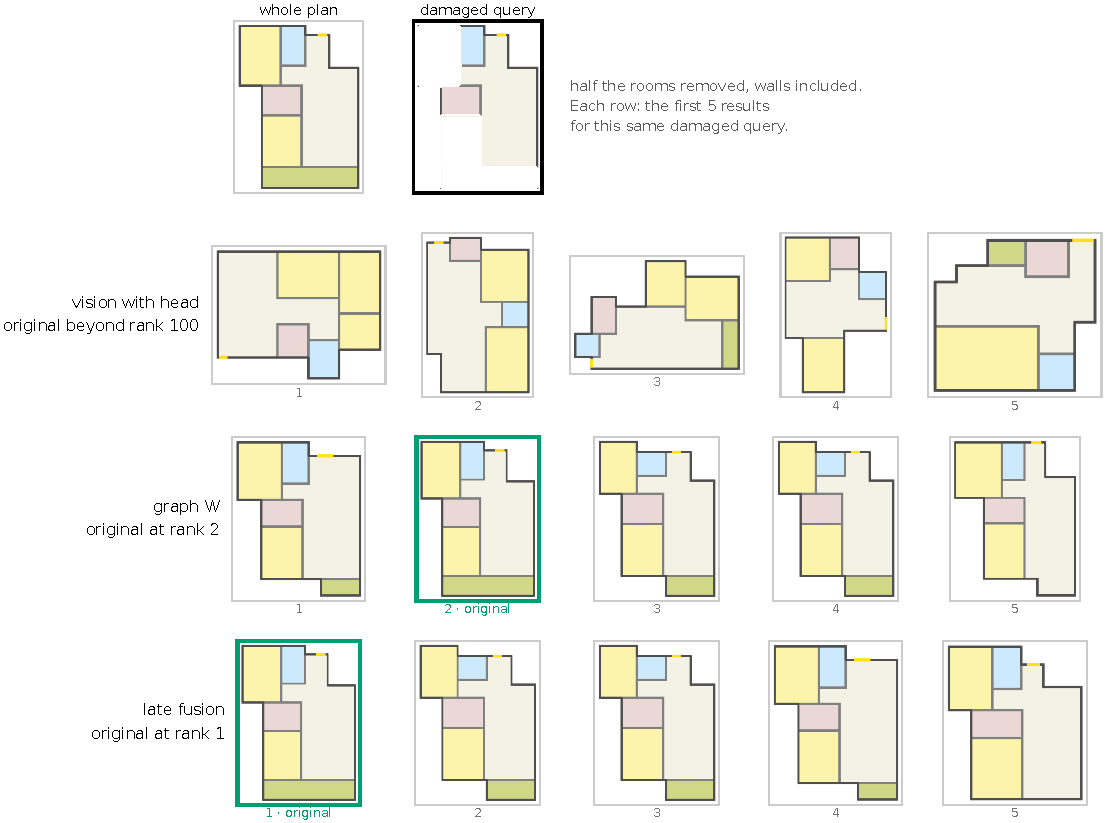
\includegraphics[width=\linewidth]{figures/english/f_final_teaser_valid.pdf}
  \caption{\textbf{Retrieving a plan from half of its rooms.}
  Top 5 of each system for one validation query; a frame marks the source.
  The single-damage vision head misses it, the graph ranks it second behind a near-identical plan, and the fusion ranks it first.
  The query is the first, alphabetically, of the 34 validation queries at this level where only the fusion ranks the source first.}
  \label{fig:teaser}
\end{figure}

% Stakes: architects search precedents from partial layouts.
Architects rarely start from a complete floor plan.
They sketch a few rooms, fix an outline or reuse a fragment of an existing plan, and then look for complete plans that contain it.
A retrieval system for this workflow must rank a large collection of plans from an \emph{incomplete} query and still find the plan the fragment came from.

% Problem gap: two structural limitations of current practice.
Two gaps separate current methods from this workflow.
First, floor-plan similarity methods learn and evaluate on complete plans: LayoutGMN~\cite{patil2021layoutgmn} and LayoutGKN~\cite{vanengelenburg2025layoutgkn} learn a structural similarity between complete RPLAN plans and score it with triplet accuracy or precision among their own top results.
Partial plans appear in floor-plan generation~\cite{hu2020graph2plan,zeng2026plancraft}, and we found no retrieval method that takes them as queries.
Second, a plan exists both as an image and as a graph of rooms, and fusing the two looks attractive because they fail in different ways: the image keeps the outline of a missing room, while a partial graph is the plausible complete graph of many smaller plans.
Yet any fusion of two models with partly independent errors gains accuracy; a fusion gain alone cannot tell whether the image adds information the graph lacks or merely acts as a second model.

% Key abstraction: ensemble controls and the complementarity gain.
We separate the two with \emph{ensemble controls}: we fuse the graph with a second model that holds the same information, either a second training of the same graph encoder or another graph encoder.
We call \emph{complementarity gain} (CG) the part of the vision--graph gain that the stronger control does not reach.
A positive CG means the image contributes information of its own.

% Design intuition.
FusePlan has two retrieval branches over the same gallery of 67{,}405 RPLAN plans~\cite{wu2019rplan} (\cref{fig:pipeline}).
The graph branch is a GATv2 encoder~\cite{brody2022gatv2} trained to map a plan with rooms removed onto the complete plan, with the checkpoint chosen on retrieval robustness.
The vision branch is a frozen PE-Spatial encoder~\cite{bolya2025perception} with whitening, optionally followed by a head trained on the same damages.
A late fusion with a single weight combines their cosine similarities.
We measure robustness as the self-recovery of the source plan when we remove rooms, a region or image patches, choose everything on validation and read the test split with the predictions written in advance.

% Results preview.
On the test split, the graph branch recovers the source with an AUC of 0.903, against 0.611 for LayoutGKN retrained on the same task.
Fusing it with the frozen image encoder adds $+0.013$, a gain that a second graph model matches; fusing it with a damage-trained vision head adds $+0.031$ (\cref{fig:teaser}), and over four replicas the damage-trained heads exceed both controls by $+0.012$ to $+0.022$.
The fusion gain follows an inverted U in the strength of the graph: it peaks at $+0.198$ when the two branches are equally strong, where even the frozen encoder passes both controls.

\noindent We make the following contributions:
\begin{itemize}
  \item \textbf{Graph branch for incomplete plans.} Training on damaged--complete pairs and selecting on robustness, after the same search over GCN, GraphSAGE and GATv2, brings self-recovery under room removal to $0.904\pm0.001$ on test, $0.29$ above a retrained LayoutGKN.
  \item \textbf{Ensemble controls and complementarity gain.} With a strong graph, a frozen image encoder adds no information beyond an ensemble effect, while damage-trained vision heads do; even then the control accounts for about half of the fusion gain, and the CG appears only where the graph has little left.
  \item \textbf{Relative strength.} Across 37 graphs, the fusion gain peaks when the branches are equally strong and shrinks near the ceiling, which reconciles a $+0.17$ gain in an earlier version of our pipeline with $+0.013$ here.
  \item \textbf{Protocol and negative results.} A self-recovery protocol with three damages, paired intervals, replicas and pre-registered test readings, and the failures that shaped it: a rendering artifact, a head that learns only the damage it sees, and a graph that collapses with symmetric pairs.
\end{itemize}

\section{Related Work}
\label{sec:related}

\paragraph{Floor-plan datasets.}
\TODO{RPLAN; CubiCasa5K, ResPlan (out of scope, future work).}

\paragraph{Graph representations and generation of floor plans.}
\TODO{Graph2Plan and related graph-based layout models.}

\paragraph{Floor-plan retrieval and similarity.}
\TODO{LayoutGMN, LayoutGKN (graph similarity on RPLAN); other floor-plan CBIR.}

\paragraph{Visual foundation encoders.}
\TODO{The eight frozen encoders of the ablation; PE-spatial for the final config.}

\paragraph{Graph neural networks and contrastive learning.}
\TODO{GCN, GraphSAGE, GATv2; InfoNCE.}

\section{Method}
\label{sec:method}

\begin{figure*}[t]
  \centering
  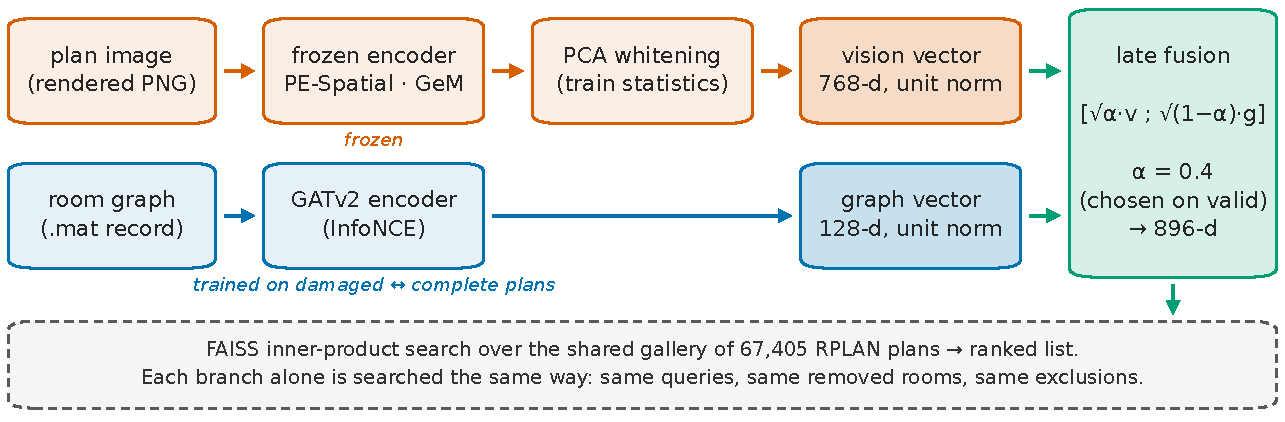
\includegraphics[width=\textwidth]{figures/english/f_final_pipeline_readme.pdf}
  \caption{\textbf{FusePlan pipeline.}
  The vision branch embeds the rendered plan with a frozen encoder and whitening; the graph branch embeds the room graph with a GNN trained to map partial plans onto complete ones.
  Late fusion concatenates the two unit vectors with weights $\sqrt{\alpha}$ and $\sqrt{1-\alpha}$ ($\alpha=0.4$ with the frozen branch, chosen on validation), so one inner product scores both.
  The damage-trained vision variants (\cref{sec:method_vision}) add a trained head to the vision branch and choose their own $\alpha$ with the same rule.
  An exact inner-product FAISS search ranks the gallery of 67{,}405 plans with the fused vector; each branch alone is searched the same way, with the same queries and removed rooms.}
  \label{fig:pipeline}
\end{figure*}

% Sources (paper-comp/CVCS-AI-Assisted-ID/): PAPER.md §5.1, §5.5-§5.8;
% fusion src/evaluation/{query_vectors,late_fusion,fusion_select}.py;
% weights results/csv_final/{valid,test}_seeds.csv (alpha_main 0.4 in 4/4, alpha_head 0.3/0.4),
% results/csv_multiseed/head_v2_fusion.csv (0.6/0.6/0.5/0.5);
% graph configs/graph_models/gat.yaml, results/csv_final/valid_graph_selection.csv (gat/comb, 317952 params);
% vision configs/vision_models/pespatial.yaml, src/vision/models/vision_encoders/base.py:10-12 (clamped GeM).
% alpha rule src/evaluation/fusion_select.py:106-130 (ties, median, closer to 0.5); ties [0.3, 0.4] in
% results/final_pipeline/fusion/s*/select_valid.json; curve grid src/evaluation/fusion_curve.py:43,135-136; heads src/vision/models/projection_head.py
% (single-damage 768->1024->256, configs/vision_retrieval.yaml:30-33; multi-damage residual 768->1024->768);
% graph out_dim 128 in configs/graph_models/*.yaml, no variant of src/graph/final_graph_configs.py changes it.

Let $\mathcal{G}$ be a gallery of floor plans, each available as a rendered image and as a structural record (room types, room boxes, typed adjacencies).
A query $\tilde{q}$ is a plan $q\in\mathcal{G}$ with part of its content removed (\cref{sec:metrics}).
The task asks for a ranking of the whole gallery that places the source plan $q$ as high as possible.
A vision encoder maps a plan to a unit vector $v$ ($v\in\mathbb{R}^{768}$ for the frozen branch, $\mathbb{R}^{256}$ for the single-damage head of \cref{sec:method_vision}) and a graph encoder maps it to a unit vector $g\in\mathbb{R}^{128}$, the size shared by every graph encoder we train.
Both branches index the same gallery and receive the same damaged queries, so we compare branches and fusions query by query (\cref{fig:pipeline}).

\subsection{Late fusion and ensemble controls}
\label{sec:method_fusion}

\paragraph{Fusion.}
The fused descriptor concatenates the two L2-normalised vectors with a single weight $\alpha$; for a query $q$ and a gallery plan $p$,
\begin{equation}
  \begin{gathered}
  z = \bigl[\sqrt{\alpha}\,v \,;\, \sqrt{1-\alpha}\,g\bigr],\\
  \langle z_q, z_p\rangle = \alpha\,\langle v_q, v_p\rangle + (1-\alpha)\,\langle g_q, g_p\rangle,
  \end{gathered}
  \label{eq:fusion}
\end{equation}
where $\langle\cdot,\cdot\rangle$ is the inner product, equal to the cosine similarity for unit vectors.
Hence $\lVert z\rVert=1$, and one exact inner-product FAISS search over the concatenated vectors (896-d with the frozen branch) ranks the gallery by a weighted average of the vision and graph cosine similarities, with weights $\alpha$ and $1-\alpha$.
At $\alpha=1$ and $\alpha=0$ the fusion reproduces the two branches, which we use as a correctness check.
For a damaged query, both branches recompute the query vector from the \emph{same} removed rooms; gallery vectors always describe complete plans.
We choose $\alpha$ on the validation split over $\{0, 0.1, \dots, 1\}$ with a rule fixed before the runs.
The criterion is the robustness to room removal (\cref{sec:metrics}), the only damage both branches can receive.
Neighbouring weights often score almost the same, so the arg-max would pick one of them by chance.
We therefore compare every $\alpha$ with the best one on the same queries: when the 95\% bootstrap interval of their paired difference contains zero (\cref{sec:metrics}), the two count as tied, and we take the median of the tied values (of two central values, the one closer to 0.5).
For $W$ with the frozen vision branch, 0.3 and 0.4 tie in all four replicas and the rule gives $\alpha^*=0.4$; every other fusion selects its own weight with the same rule (the graphs of \cref{fig:curve} on the coarser grid $\{0, 0.2, \dots, 1\}$), and the test split uses the weights fixed on validation.
The fusion is static: every query uses the same $\alpha$, and no gate adapts the weight to the single query, for instance to how much of it is missing.

\paragraph{Ensemble controls.}
Fusing any two models with partly independent errors raises retrieval accuracy, so a fusion gain alone does not show that the image carries information the graph lacks.
We therefore compare every vision--graph fusion with two \emph{ensemble controls} that fuse the graph with a second model holding the \emph{same} information: a second training of the same graph configuration (different initialisation and batches), and a graph encoder of another family trained with the same recipe.
Each control selects its own weight on validation with the rule above.
For a fusion $F$ of branches $A$ and $B$, the per-query gain is $\mathrm{gain}_F(q)=\mathrm{AUC}_F(q)-\mathrm{AUC}_{b}(q)$, where $b$ is the branch with the higher mean AUC.

\paragraph{Complementarity gain.}
We call \emph{complementarity gain} the part of a vision--graph gain that no second graph model provides,
\begin{equation}
  \mathrm{CG} = \overline{\mathrm{gain}}_{V+G} - \overline{\mathrm{gain}}_{C^\star},
  \label{eq:cg}
\end{equation}
where $C^\star$ is the ensemble control with the larger mean gain, a conservative choice.
We compute CG query by query, on the same queries for both fusions, with a 95\% bootstrap interval (\cref{sec:metrics}).
$\mathrm{CG}>0$ means the vision branch contributes information beyond an ensemble effect; the remaining part $\overline{\mathrm{gain}}_{C^\star}$ is what a second graph model would already deliver.
The two parts come from different fusions, so they summarise the gain and do not split one fusion additively.

\subsection{Graph branch}
\label{sec:method_graph}

\paragraph{Room graph.}
We build each graph from the RPLAN record~\cite{wu2019rplan}, not from the image.
Each room becomes a node whose 19 features concatenate a one-hot encoding of the 13 room types with the centre, width, height, area and aspect ratio of the room box on the $256\times256$ RPLAN grid; we clip the aspect ratio at its 99th percentile and standardise the geometric features.
Each adjacency becomes an undirected edge with a one-hot encoding of the 10 RPLAN relation types.

\paragraph{Encoder.}
The encoder $W$ stacks three GATv2 layers~\cite{brody2022gatv2} with hidden size 256, one attention head and edge features in the attention.
We sum-pool the node states and concatenate the sum-pooled input features; on the one-hot part this skip connection equals the room-type histogram.
A linear layer projects the result to 128 dimensions, followed by L2 normalisation (317{,}952 parameters).

\paragraph{Training for incompleteness.}
We train with the symmetric InfoNCE loss~\cite{oord2019cpc}, in-batch negatives, temperature $\tau=0.1$, batch size 256, learning rate $10^{-3}$, weight decay $10^{-5}$ and no dropout, on the training split only.
Positive pairs are \emph{asymmetric}: one view is the complete plan, the other removes a fraction $f\sim\mathcal{U}[0.25,0.75]$ of its rooms together with their edges.
The pair thus asks the encoder to map a partial plan onto its complete version, the retrieval task itself.
We select the checkpoint on retrieval, not on the loss: after each epoch we measure the robustness to room removal on 2{,}000 validation queries disjoint from the evaluation queries, with the whole gallery, over 600 epochs.
The selected epoch falls between 550 and 592 in all four replicas, so the reported robustness of the graph is a lower bound.

\paragraph{Configuration search.}
We chose $W$ with the same recipe for GCN~\cite{kipf2017gcn}, GraphSAGE~\cite{hamilton2017graphsage} and GATv2.
Starting from a reference configuration per encoder, we changed one factor at a time: temperature, skip connection, rotation and reflection augmentation, a lost-neighbour marker, depth, width, pooling, aggregator and attention heads.
We then combined the changes that improved robustness in all four seeds.
We train each of the 37 candidates with 4 seeds and score it on validation only (\cref{tab:ablation_graph}).
$W$ is the combination for GATv2: $\tau=0.1$, no rotations or reflections, three layers, width 256 and one head.

\subsection{Vision branch}
\label{sec:method_vision}

\paragraph{Frozen encoder.}
The vision branch uses the spatially aligned Perception Encoder~\cite{bolya2025perception} (PE-Spatial, ViT-B/16) without training.
We resize the rendered plan so that its longer side has 224 pixels, keeping the aspect ratio, and pad it to a square with the white background.
The descriptor is the generalised mean (GeM~\cite{radenovic2019gem}) with $p=3$ of the last-layer patch tokens $x_1,\dots,x_N$, computed per channel as $\bigl(\tfrac{1}{N}\sum_i \max(x_i,\epsilon)^p\bigr)^{1/p}$ with $\epsilon=10^{-6}$.
The clamp at $\epsilon$ comes from the standard GeM implementation, designed for CNN activations that are non-negative after the ReLU.
ViT tokens after the final LayerNorm are signed, so here the clamp zeroes their negative components and the descriptor pools only the positive part of each channel.

\paragraph{Whitening and indexing.}
We apply PCA whitening~\cite{jegou2012whitening}: mean and covariance come from training-split plans only, and every descriptor $x$ maps to $\Lambda^{-1/2}U^\top(x-\mu)$, keeping all 768 components, followed by L2 normalisation.
An exact inner-product FAISS index~\cite{douze2025faiss} stores the gallery.
Whitening matters because the frozen descriptors of the synthetic renderings collapse into a narrow cone; it improves robustness in all 26 encoder, pooling and resolution settings we tested (\cref{tab:ablation_vision}).
PE-Spatial with this pooling and whitening is the most robust of 52 frozen configurations over 8 encoders~\cite{oquab2024dinov2,simeoni2025dinov3,tschannen2025siglip2,ranzinger2024amradio,assran2023ijepa,cao2026tipsv2,bolya2025perception}, selected on validation.

\paragraph{Damage-trained heads.}
To test whether a vision branch trained on the damage carries more information, we train two alternative heads on top of the frozen encoder; each one replaces the frozen branch in its own fusion, and the two are never stacked.
Both train with InfoNCE ($\tau=0.07$, batch 4{,}096) on training plans, with self-supervised positives and no relevance labels.
The \emph{single-damage head} is an MLP ($768\to1024\to256$, GELU) applied to gallery and queries; it learns to match a plan with rooms removed to the complete plan, and we re-estimate the whitening on its 256-d outputs.
The \emph{multi-damage head} acts on queries only: it adds a residual MLP ($768\to1024\to768$, last layer initialised at zero) to the whitened frozen vector, so the gallery stays frozen; it trains on room removal, crop and patch in turn.
Both heads select their epoch on 1{,}000 validation queries disjoint from the evaluation queries.

\section{Experiments and Results}
\label{sec:experiments}

\subsection{Metrics}
\label{sec:metrics}

\paragraph{Incomplete queries and robustness metric.}
\TODO{Three damages at $f\in\{0.25,0.5,0.75\}$: rooms removed with their walls, crop, patch. Self-recovery reciprocal rank $\rightarrow$ AUC over levels $\rightarrow$ $R$ = mean of the three AUCs. Paired bootstrap 95\% CI. PAPER.md \S5.4; project status.md \S38.}

\paragraph{Per-axis relevance (descriptive).}
\TODO{Composition, topology, geometry; nDCG@10 on the full plan. Descriptive only: circular on every axis. PAPER.md \S5.2--\S5.3, \S5.5.}

\subsection{Dataset and experimental details}
\label{sec:setup}
\TODO{Table T1: RPLAN, official splits, shared gallery, 2000 queries (seed 42), valid selects, test read once, exclusions, random floor. Project status.md \S20, \S29.}

\subsection{Results}
\label{sec:results}

\subsubsection{Ablation}
\label{sec:ablation}
\TODO{Ablation table (mean $\pm$ std, pending D1): vision configurations under the three damages; graph; fusion weight $\alpha$ and the two controls. Main test result (T3, project status.md \S53).}

\begin{figure}[t]
  \centering
  \includegraphics[width=\linewidth]{figures/f_damage_test.pdf}
  \caption{\TODO{Test split: self-recovery vs.\ fraction of removed rooms for hist, vision, graph and fusion. Source: f\_damage\_test.sources.txt.}}
  \label{fig:damage_test}
\end{figure}

\begin{figure}[t]
  \centering
  \includegraphics[width=\linewidth]{figures/f_alpha_valid.pdf}
  \caption{\TODO{Valid split: robustness AUC vs.\ $\alpha$ for the three fused pairs. Source: f\_alpha\_valid.sources.txt.}}
  \label{fig:alpha}
\end{figure}

\paragraph{Negative results.}
\TODO{Wall artifact of the historical room masking (project status.md \S35--\S37); the trained projection head does not transfer to other damages (\S37, \S48); the lost-neighbours marker ties (\S47).}

\begin{figure*}[t]
  \centering
  \includegraphics[width=\textwidth]{figures/f_damage_kinds_valid.pdf}
  \caption{\TODO{Left: final vision config under the three damages. Right: the wall artifact, same removed rooms with walls kept or erased. Source: f\_damage\_kinds\_valid.sources.txt.}}
  \label{fig:damage_kinds}
\end{figure*}

\subsubsection{Qualitative results}
\label{sec:qualitative}
\TODO{Qualitative examples by model and on the dataset (\cref{fig:teaser}).}

\section{Conclusions}
\label{sec:conclusion}
\TODO{Summary; limitations (PAPER.md \S8: RPLAN only, synthetic damages, proxy relevance, fusion tied to this graph checkpoint); future work (PAPER.md \S9).}

{
    \small
    \bibliographystyle{ieeenat_fullname}
    \bibliography{main}
}

% WARNING: do not forget to delete the supplementary pages from your submission 
% \clearpage
\setcounter{page}{1}
\maketitlesupplementary

\section{Additional figures}
\label{sec:suppl_figures}

\begin{figure}[h]
  \centering
  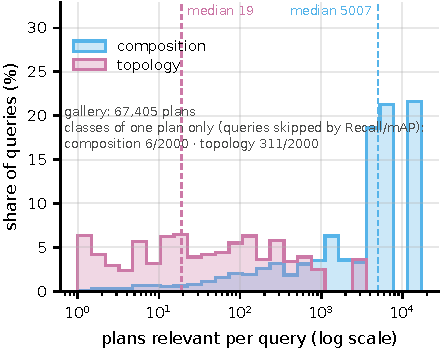
\includegraphics[width=\linewidth]{figures/english/f_classes_valid.pdf}
  \caption{\TODO{Size of the equivalence classes, composition vs.\ topology. Source: f\_classes\_valid.sources.txt.}}
  \label{fig:classes}
\end{figure}

\begin{figure*}[h]
  \centering
  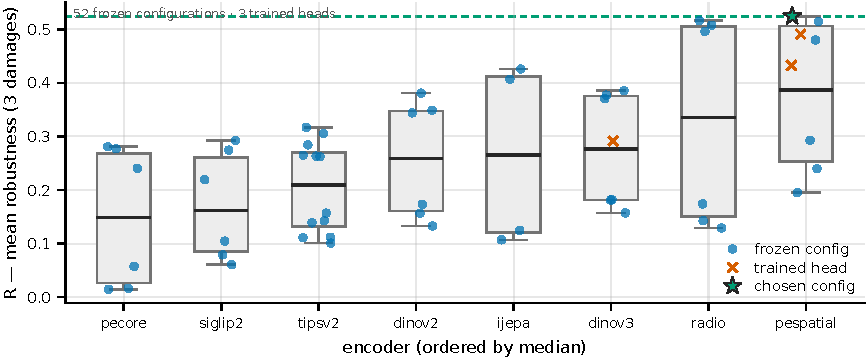
\includegraphics[width=\textwidth]{figures/english/f_ablation_valid.pdf}
  \caption{\TODO{Robustness $R$ of every configuration, grouped by encoder. Source: f\_ablation\_valid.sources.txt.}}
  \label{fig:ablation_box}
\end{figure*}


\end{document}
